
\chapter{Task A}
\section{Environment description}
The environment is implemented as a weighted, un-directed graph, figure
\ref{fig:graph}.  The graph consist of Vertices(figure \ref{fig:uml_vert}) and
Edges(figure \ref{fig:uml_edge}) that is connected to each other.  By doing this
we can let the agent traverse the graph by itself using an implementation of the
shortest path algorithm as the heuristic for the A* algorithm to select the next
move to make. 

The environment also contains the possibility for marking edges as broken,
vertices as visited, and creating edges between Vertices.

\begin{figure}[h]\centering
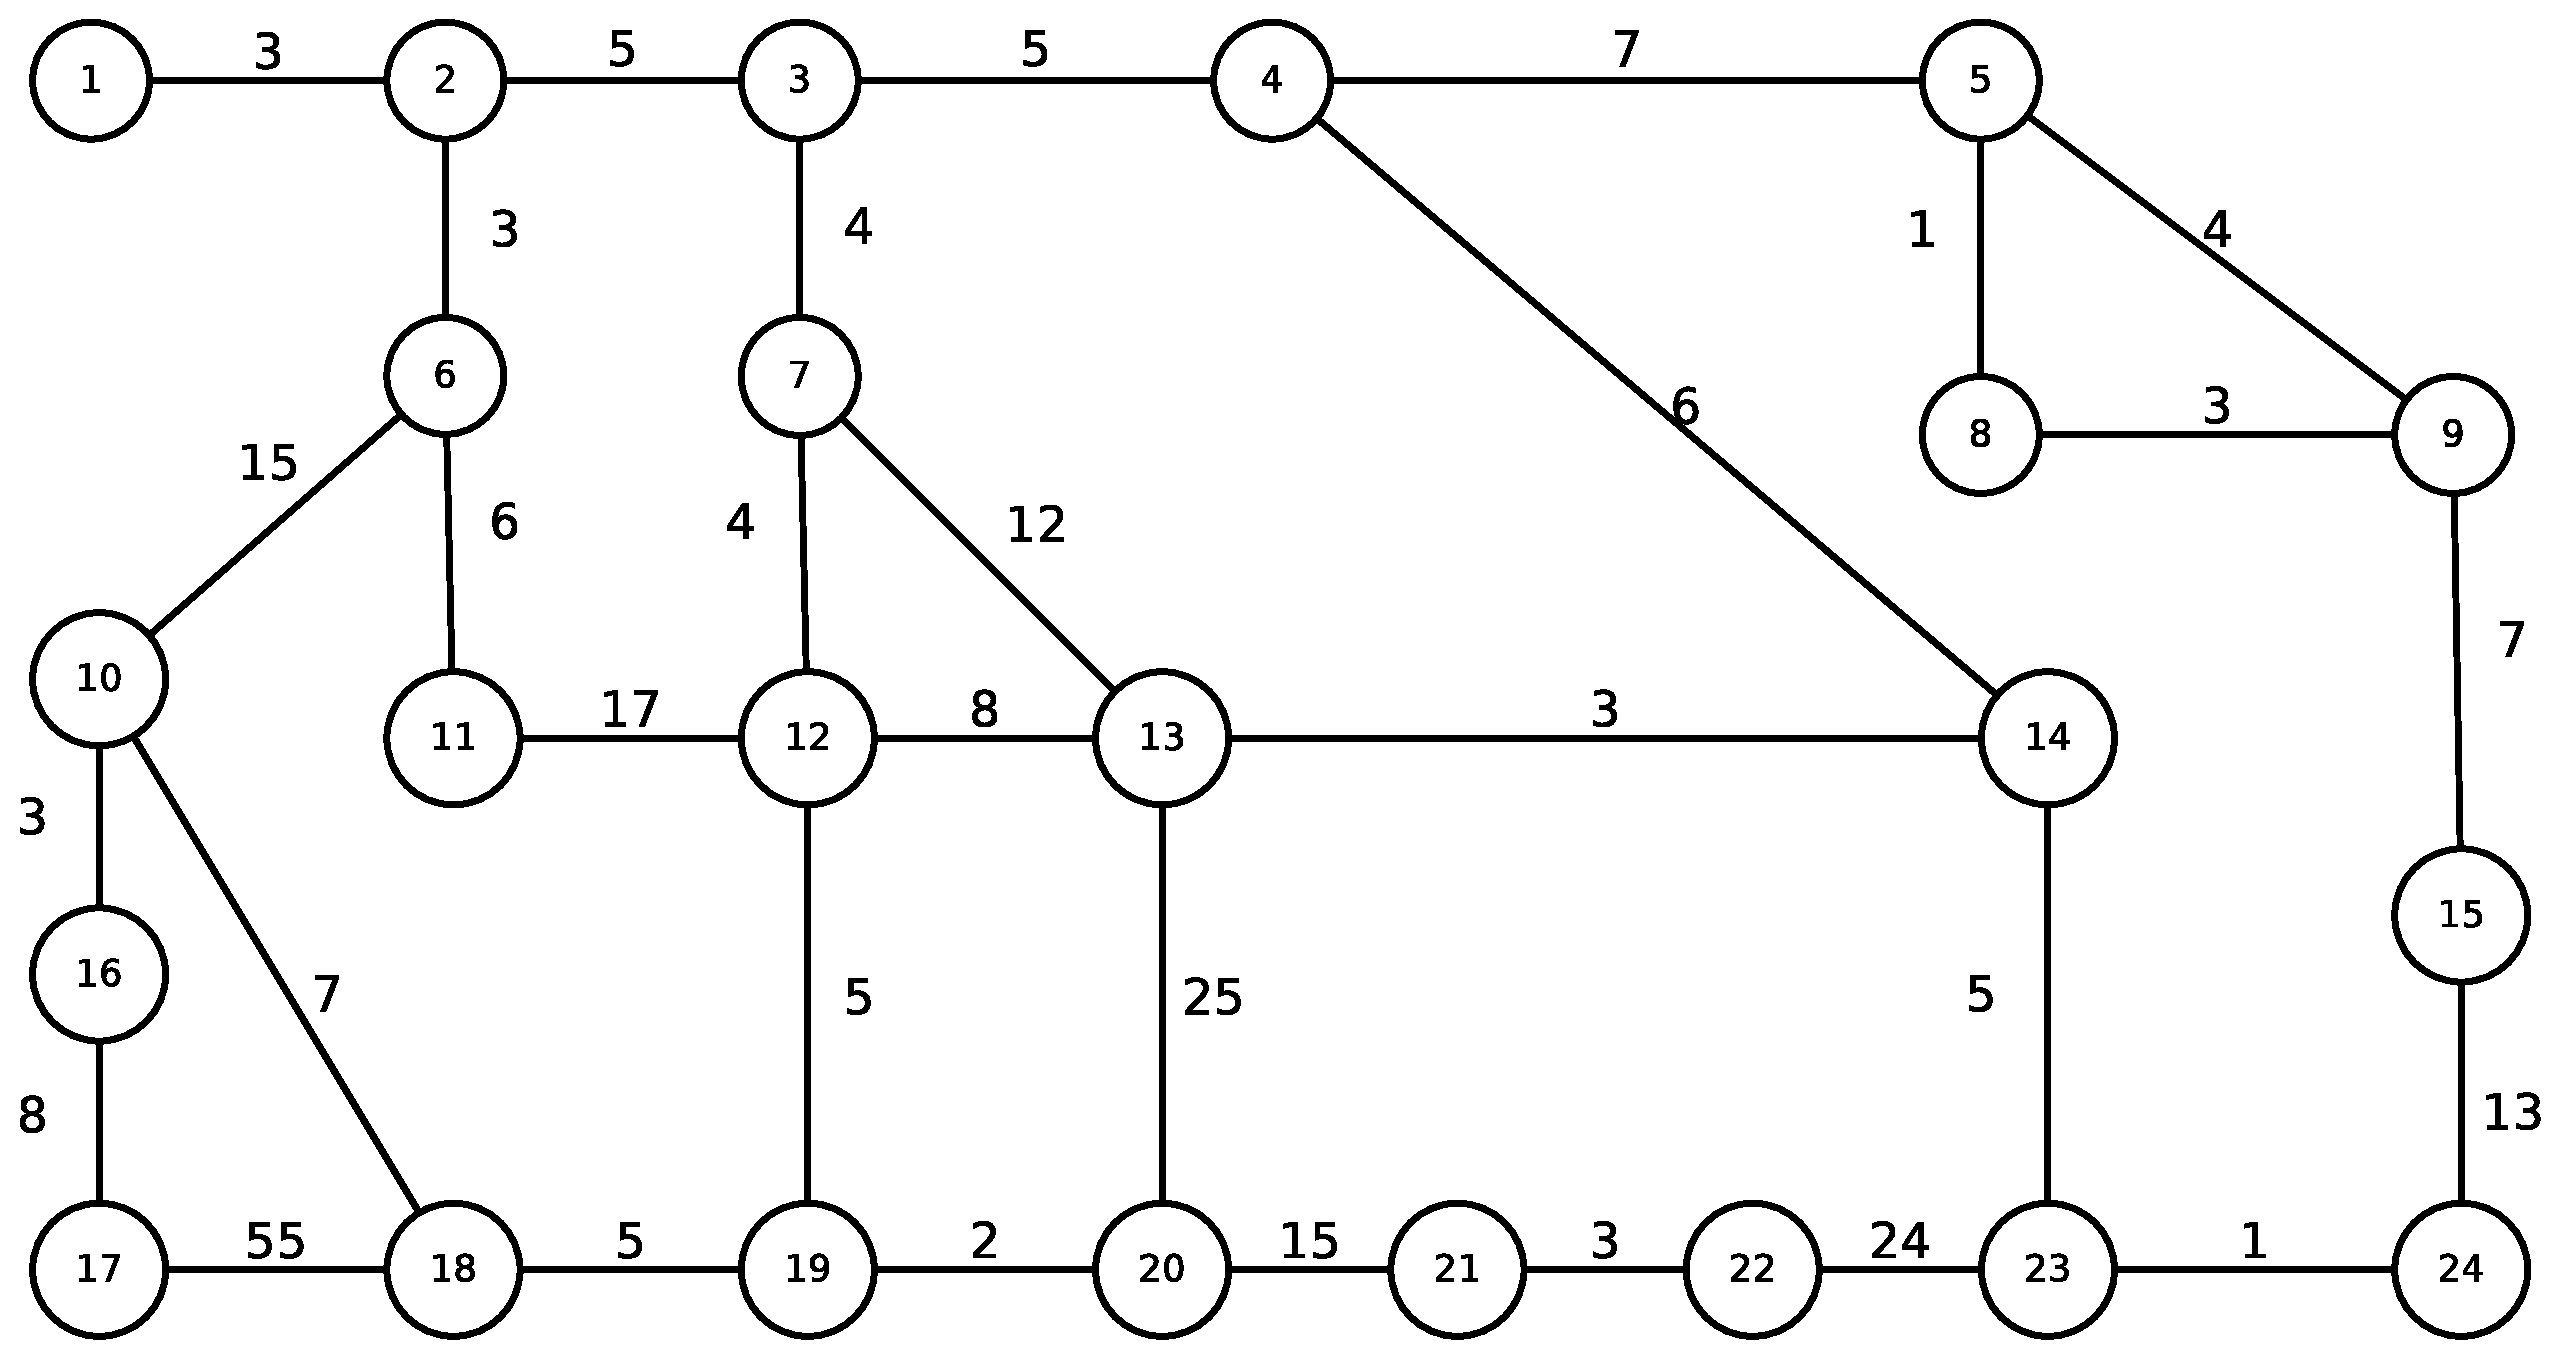
\includegraphics[ width={0.7\textwidth} ]{pictures/graph}
\caption{The environment - A non-directed graph with weighted edges.}
\label{fig:graph}
\end{figure}


\subsection{Vertice}
Vertices are the junctions in graph in which the agents travels from and to
using the edges. The Vertices holds no significant value other than being the
agent's goal and intermediate locations. The vertices are connected to eachother
using edges. The Vertices consists of the following variables and functions as
depicted in the UML-class in figure \ref{fig:uml_vert}.

\begin{description}
\item [key:]			This is an integer value holding the reference key to the
	Vertice. It is assigned automatically during creation of the vertice using an
	auto incremented counter starting at 1.  This is used to identify a specific
	Vertice in the graph and the vertice list.
\item [name:]			This is an unused variable and is assigned to NULL during
	creation. It is meant to hold a small text describing the name of the Vertice,
	and is usefull if it the graph represents a map or other things that could be
	assigned a description using a name tag.
\item [visited:]	This is a boolean describing wether or not the Vertice has
	been visited. It is not currently used, but could be used to mark a cell as
	visited during traversal.
\item [nxtVert:]	This is a pointer to a Vertice object. This will point to
	either the next Vertice in the list or to the vTail object which represents
	the end of the vertice list.  For vTail this link will link back to itsself.
\item [eStart:]		This is an Edge pointer which is on construction initialized
	to an Edge object that points to NULL.  This edge is the starting element for
	the list of Edges stemming from the current Vertice to adjacent vertices.
	eStart is however a dummy-element that points to the first actual edge in the
	list.
\end{description}

\begin{figure}[h]\centering
	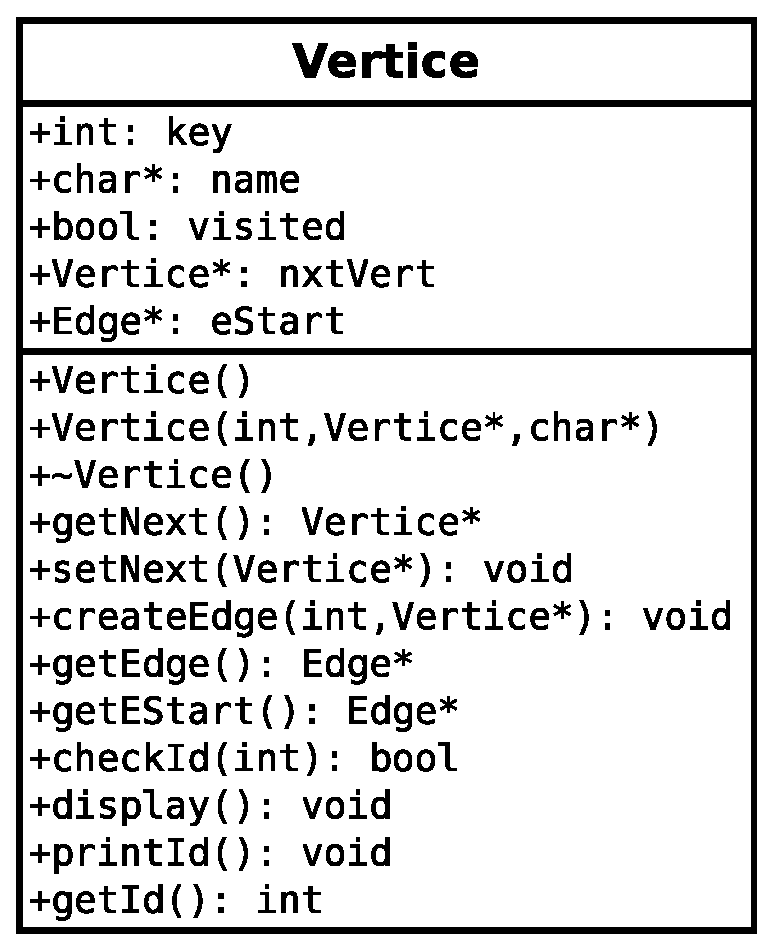
\includegraphics[ width={0.35\textwidth} ]{pictures/uml_vertice}
	\caption{UML description of a Vertice's variables and implemented functions}
	\label{fig:uml_vert}
\end{figure}




\subsection{Edge}
The edge objects depicts the links between vertices in the graph. Each vertice
is in charge of its own links to neighboring cells, which in turn requires that
the number of edges in the environment is $2E$.  Since it is un-directed the
vertices at both end points of the edge has to have a link to eachother.

This could be avoided by having a separated edgelist with pointers to both
vertices connected to the edge, but it would drastically increase search time.
In larger graphs it would maybe be mor feasable since it would require less
memory.

\begin{description}
\item[status:]	This boolean value holds the status of the edge, which means 
	whether or not it	is traversable.  This could be used to update the 
	environment dynamically runtime.
\item[cost:]		This is the integer value representing the cost of traveling the
	edge from current vertice to the linked vertice. This is the value used to
	calculate the heuristic of path costs.
\item[nxt:]			This is the a pointer to the next Edge in the edge list. The
	first edge in the list will be the dummy edge and the last element will point
	to NULL, which will result in a segfault if not handled properly.
\item[vert:]		This is a pointer to the linked Vertice in which the endpoint of
	the link is attached to.
\end{description}

\begin{figure}[h]\centering
	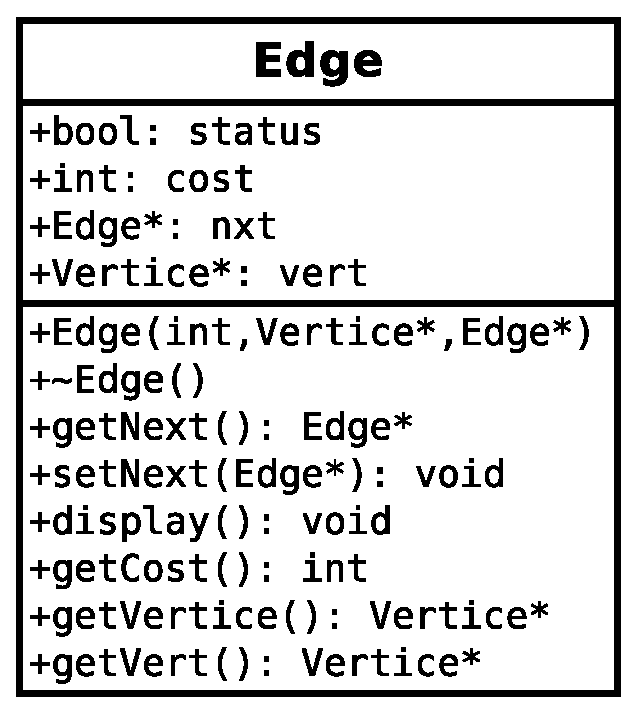
\includegraphics[ width={0.30\textwidth} ]{pictures/uml_edge}
	\caption{UML description of an Edge's variables and implemented functions}
	\label{fig:uml_edge}
\end{figure}



\subsection{Graph Construction}
As the program starts up we read the file "vertice.lst" which contains a number
stating how many vertices are going to be in the graph. After reading this
integer it continue with creating the vertices and adding them to our Vertice
list, figure \ref{fig:vert_list}, see section \ref{sec:vert_list} for details.

When all vertices are created we continue by reading the edge descriptions from
the file. The file format for edges are three integers representing the
following; "[START VERTICE ID]" "[END VERTICE ID]" "[TRAVEL COST]".

After reading the values we search using the "\textsc{findVertice( int )}"
function to find the two vertices and call the vertice function
"\textsc{createEdge(int, Vertice*)}". This will then create an edge from the
first vertice retrieved, with the specified cost that links to the other
retrieved vertice which is sent as a parameter. 

After creating the first edge it will create the second edge back to the first
vertice. Vertices is created in an unorganized list using a FIFO list.

After creating the environment one is left with a two structures, one being the
graph, figure \ref{fig:graph}, and the vertice list, figure \ref{fig:vert_list}.
Both structures consists of linked Vertice objects as shown in figure
\ref{fig:vert_struct}.

\begin{figure}[h]\centering
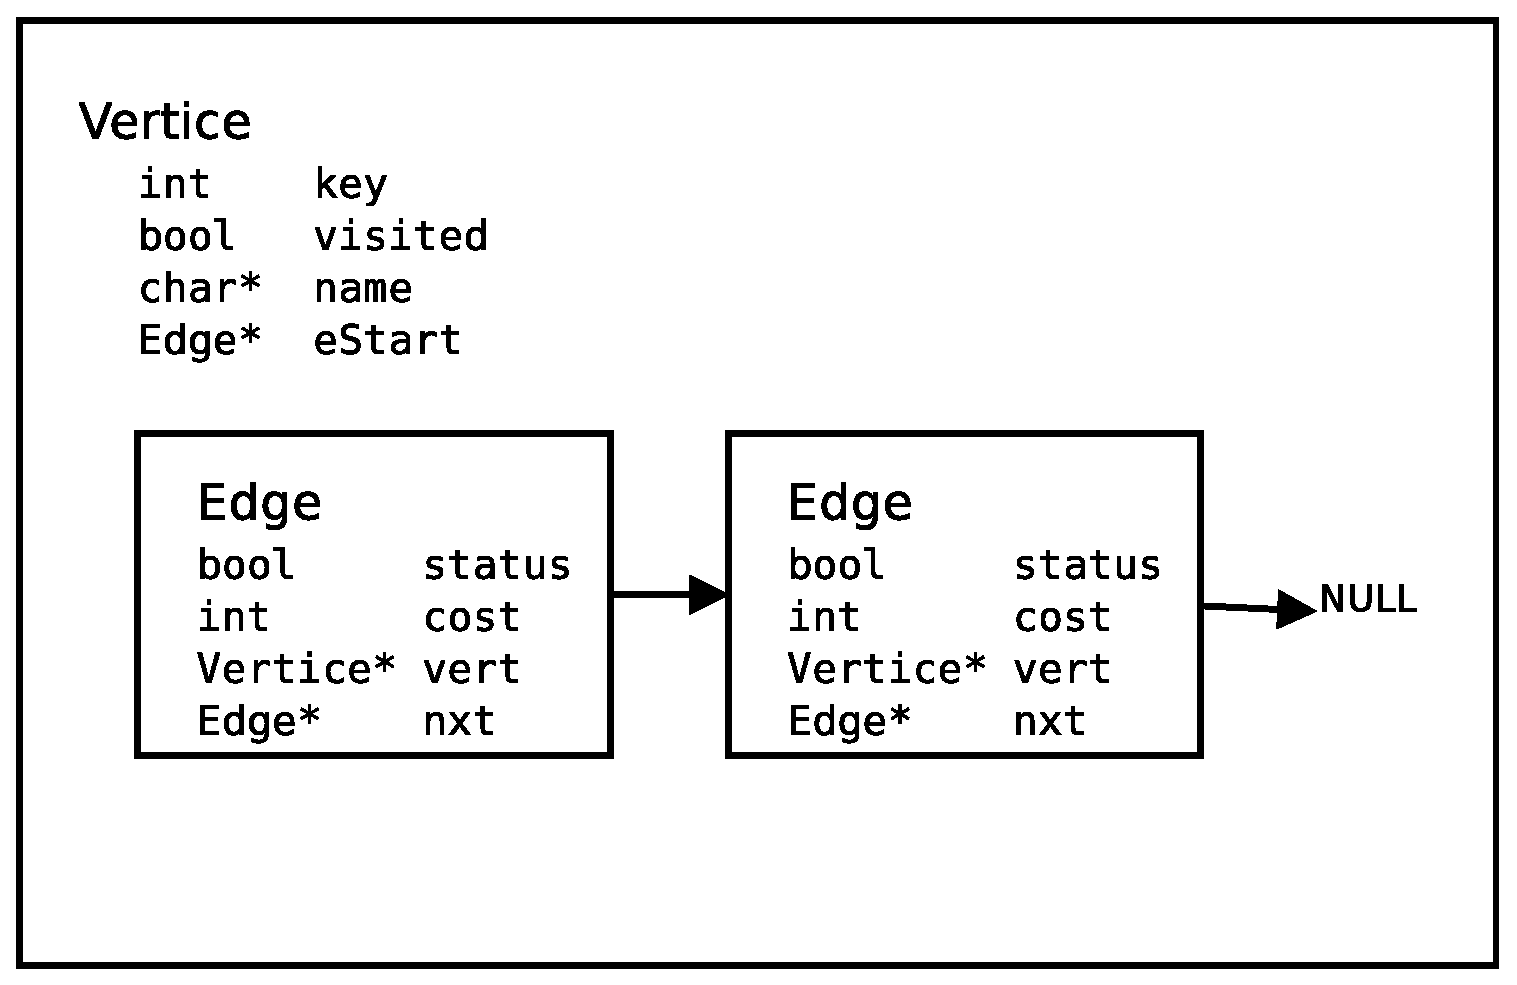
\includegraphics[ width={0.50\textwidth} ]{pictures/data_structure}
\caption{Illustration of the structure of a Vertice object}
\label{fig:vert_struct}
\end{figure}



\subsection{Vertice List}\label{sec:vert_list}
The vertice list is a list of Vertice objects where each Vertice is linked to
the next forming a FIFO\footnote{FIFO - First In First Out } list.  This list is
held on to by using two declared variables called "vStart" and "vTail". 

These two variables are two Vertice objects with no real information and are
only used as a start and end point for the list. 

The vTail element is used as to indicate the end of the list and it links back
to itsself to avoid going into a corrupt memory address during traversal. The
vStart will provide a handle to the list so one can start searching from the
front of the list.

The list is a single link chain, meaning the elements in the list only link two
the next item and not back to the previous item.

Each Vertice in the list has an internal list starting with the eStart variable,
an Edge object that acts as the same way as vStart. It is a dummy object used
for grabbing a hold of the Edge list. Each element in this list has a pointer to
an element in the Vertice list, which indicates that the current Vertice is
linked to this vertice in the graph at the specified cost.

As shown in figure \ref{fig:vert_list}, the first vertice has to edges that
links to two other vertices in the vertice list.  Indicated by red stipled
lines.  The two linked vertice elements will both have their own edge elements
linking back to the first vertice. As indicated by the blue and black stipled
lines in the figure.

\begin{figure}[h]\centering
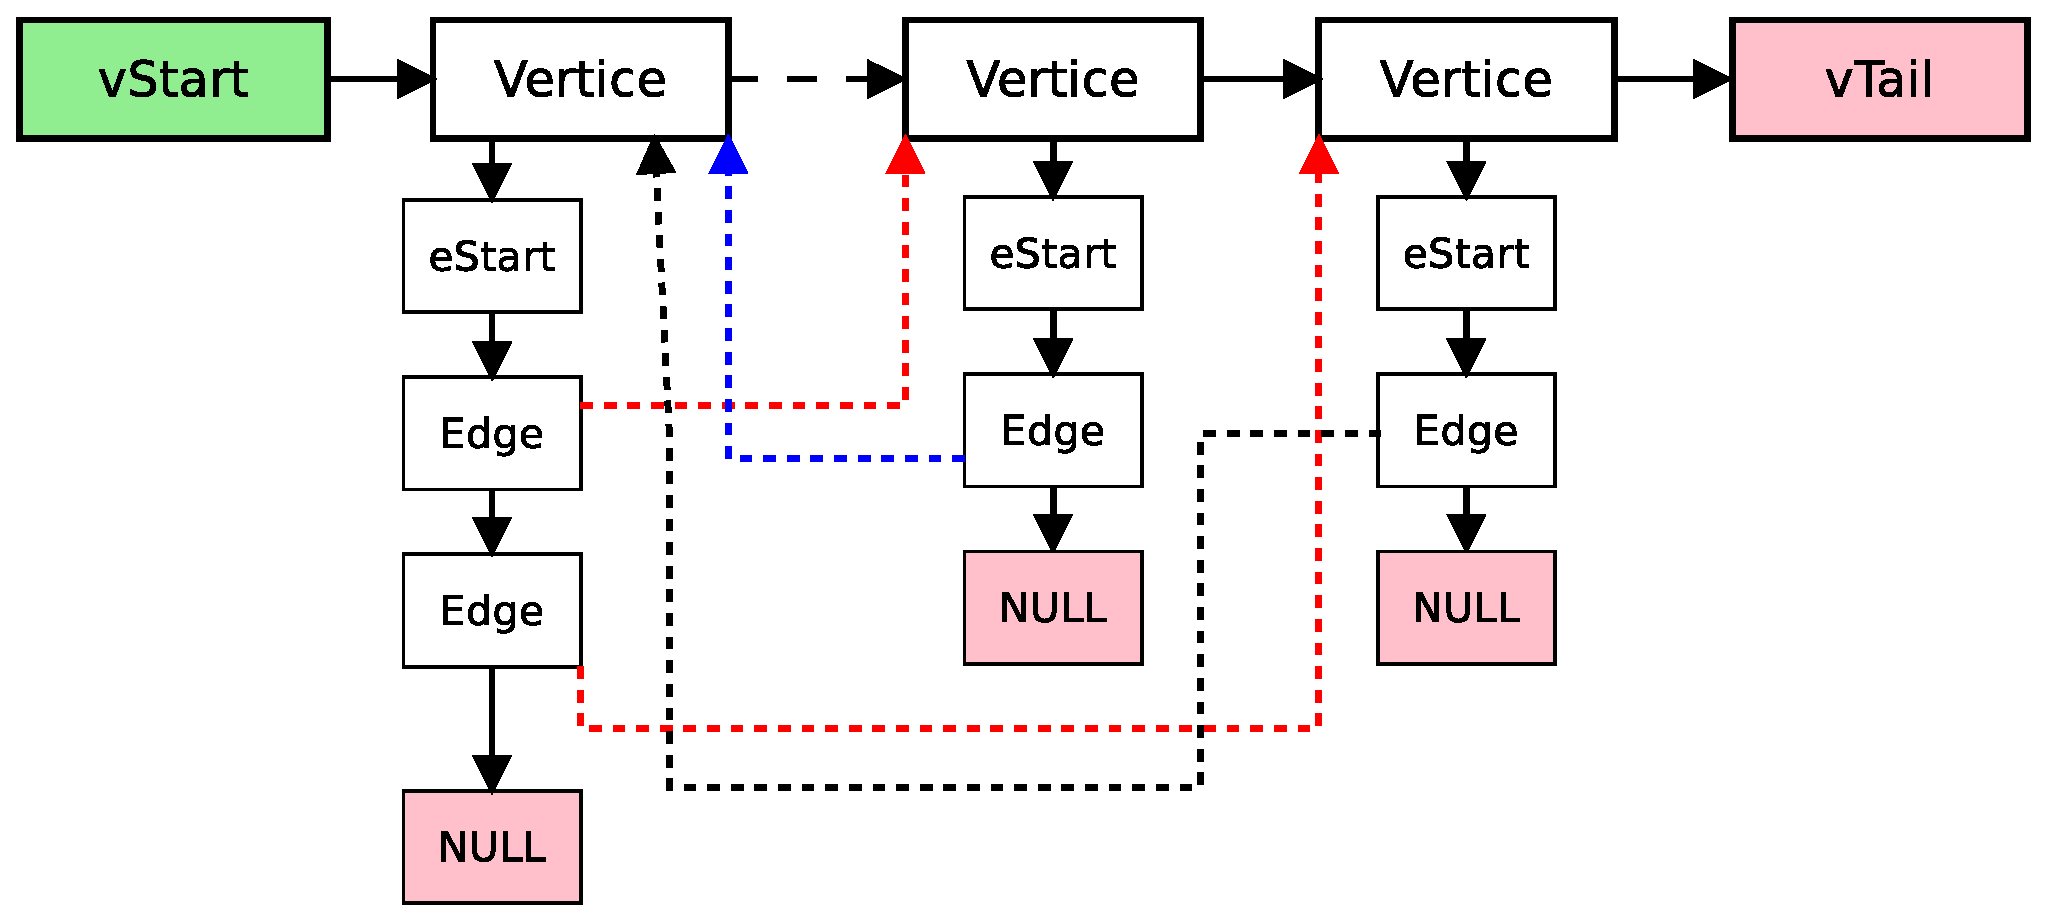
\includegraphics[ width={0.9\textwidth} ]{pictures/vertice_list}
\caption{Illustration of the list holding all the Vertices in the graph
environment}
\label{fig:vert_list}
\end{figure}



\section{Agent}
The agent is created to traverse the graph using A* tree search algorithm. It
applies this using the heuristic value by extrapolating using the shortest path
algorithm implemented in "\textsc{shp( Vertice*, int )}" to calculate the
shortest path from the upcoming Vertice to the goal. Then joining this value to 
the travel cost of getting to the upcoming Vertice.

The A* Tree search algorithm is implemented in the agent function
"\textsc{aStar()}" which creates a main fringe list, see section
\ref{sec:fringe}, "localFringe" as the open list
where it stores the frontier of un-visited vertices.  It doesn't keep track of
the vertices it has visited so it will add any node it has just traveled on onto
the fringe with an updated cost value.

The fringe is implemented as a priority queue where the edge with the lowest
estimated value are stored at the end of the list.  By turning this list around
we would reduce the search time, but the number of fringe elements to search
through isn't so large that it would matter.

The fringe elements is inserted after calculating the shortest path of the
vertice and the cost of getting to that vertice.  This total value is the total
heuristic that is taken into account of the A* algorithm.

\begin{description}
\item[goalKey:]		Integer value holding the key of the goal vertice element.
	This is used to check whether the current node is the goal state
\item[location:]	This is a Vertice pointer that holds the initial location of 
	agent.  This is used by the A* algorithm to provide the initial state of the
	agent.
\item[travCost:]	Currently unused, but its purpose is to hold the currently
	optimal travCost. Currently we are implementing this as a local variable
	instead.  travCost would be used to hold the optimal paths cost after
	finishing, but is not needed for this task.
\item[execCount:]	This is an integer value used to hold the number of executed
	lines of code. This value is used to display the time complexity of the
	algorithm instead of using the *nix time command to measure time.  This is
	because it provides a way more accurate measure of time as the computer clock
	and CPU is notoriusly unstable combination to measure time with.
\end{description}

\begin{figure}[h]\centering
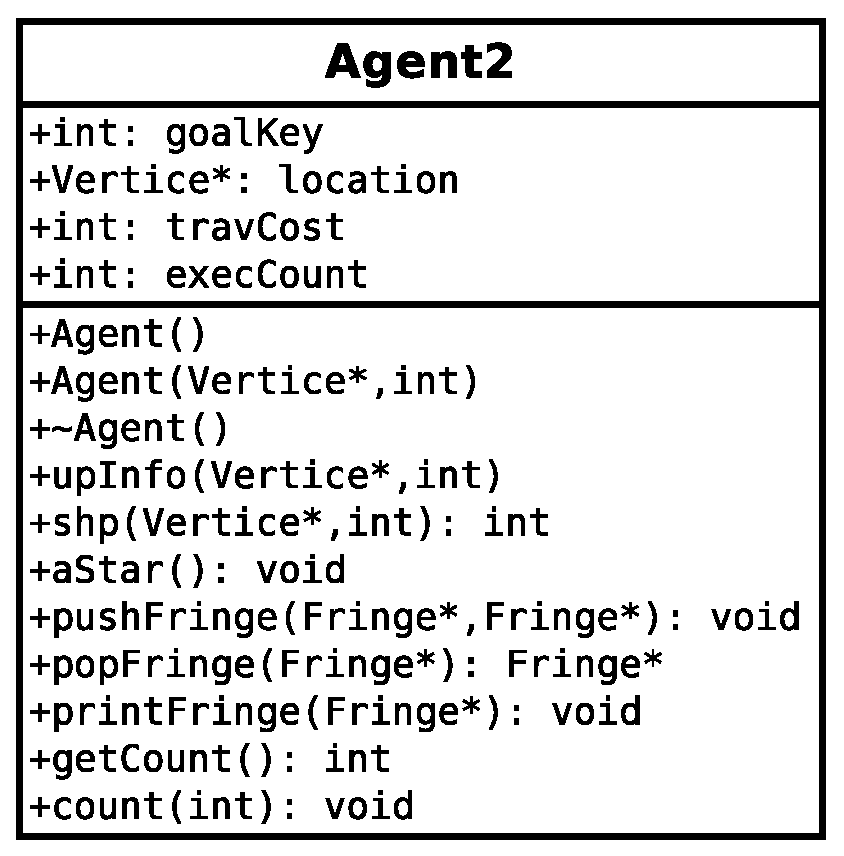
\includegraphics[ width={0.4\textwidth} ]{pictures/uml_agent2}
\caption{UML description of the Agent class, in agen2.h/cpp}
\label{fig:uml_agent}
\end{figure}



\subsection{Fringe List}\label{sec:fringe}
The fringe list is a list used to hold the information about visited and
unvisited vertices in the agents memory.

The list is implemented as a priority queue where the elements are ordered
descending according to their total heuristic value $f(n)=h(n)+g(n) => 
f(n)=estCost+travCost$. Here "estCost" is the cost of the shortest path
algorithm from the vertice to the goal and "travCost" is the sum of the path
getting from the initial location to the vertice.

The element that get retrieved from the list is allways the lowest item/the rear
item of the list.  By doing this we will always check the path with lowest total
value. either it being the A* algorithm or the shortest path algorithm.

\begin{description}
\item[travCost:]	Integer value describing the total cost of traveling to this
	Vertice from the starting point of the algorithm.  This is the sum of the cost
	of all edges traversed from initial state to current state.
\item[estCost:]		Integer value describing the estimated cost of traveling from
	this vertice to the goal state. This is estimated using the shortest path
	algorithm from the vertice in question to the goal vertice.  This will allways
	result in an admissable heuristic since it will never over estimate the lowest
	value to the goal.
\item[nxt:]				This is the link to the next element on the fringe. The last
	element will link to NULL, which must be handled correctly.
\end{description}

\begin{figure}[h]\centering
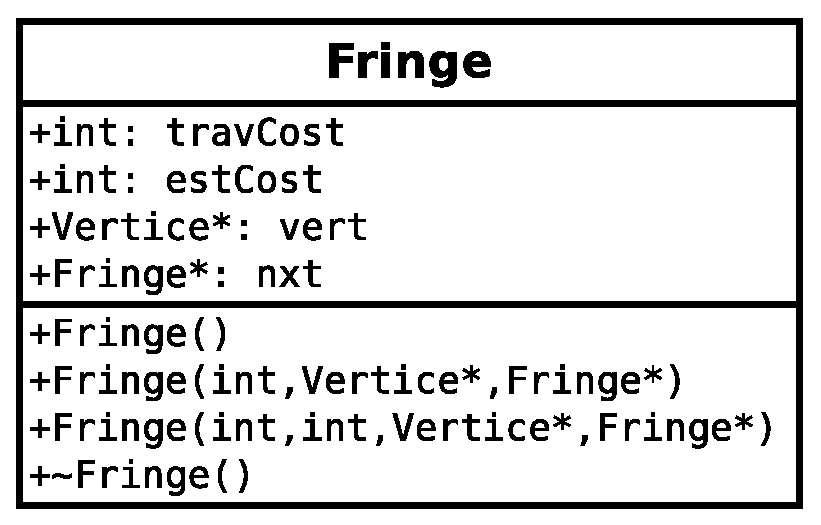
\includegraphics[ width={0.4\textwidth} ]{pictures/uml_fringe}
\caption{UML description of the Fringe object}
\label{fig:uml_fringe}
\end{figure}


\section{A* Algorithm}

\subsection{Shortest path}
The main difference between the A* and shortest path algorithm is that the
shortest path algorithm doesn't take the currently traveled cost into
consideration.  It will allways set the "travCost" value to zero and use that as
the total "travCost" up until the current vertice. The "estCost" value will be 
sum of the cost of the current path traveled.

The shortest path algorithm is as follows.
\begin{enumerate}
\item Check if current state is the goal state. If the current Vertice is the
	goal, return 0 as shortest path cost.
\item Create and add all adjacent Edges with their corresponding Vertices to the
	fringe by using the edge cost as their estCost value.
\item While fringe list is not empty retrieve the cheapest option from fringe.
	If not cheaper than current cheapest path skip the element and delete it.
\begin{enumerate}
\item Check if retrieved fringe element is the goal.  If goal state update the
	optimal path cost if new lowest value.
\item	If not goal state grab all adjacent edges from the vertice and create new
	fringe elements which are pushed to the list.  This using the current elements
	estimated cost value and new edge's cost as the new fringe elements cost.
\item delete retrieved fringe element to free up memory.
\end{enumerate}
\item clean up remaining Fringe
\item return the cheapest path cost
\end{enumerate}



\subsection{A* Tree Search}
This algorithm makes use of the value derived from the shortest path algorithm
as the heuristic.

\begin{enumerate}
\item Create open fringe to hold frontier
\item Create element from inital state and push element to open fringe.
\begin{itemize}
\item Use current location for as the vertice
\item Use zero as estimateed cost and travel cost.
\end{itemize}

\item while frontier isn't empty
\begin{enumerate}
	\item Pop cheapest element from fringe
	\item If element is the goal state, update cheapest cost and print statement
	\item If heuristic is lower than cheapest cost
	\begin{enumerate}
	\item extract vertice and travel cost from element
	\item For each edge from vertice calculate shortest path to goal state.
	\item Create new fringe elements.
	\begin{itemize}
	\item Use the current fringe elements travel cost plus the edge's cost as new 
		travel cost.
	\item Use the the shortest path value from adjacent vertice to goal as the 
		heuristic for the estimated value.
	\end{itemize}
	\item Push new elements to open fringe.
	\end{enumerate}
	\item 
	\item calculate the heuristic using the shortest path value from vertice to
		goal. Set travel cost as the edge's cost value.
	\item Create a new fringe element with the calculated heuristic.
	\item Push element to fringe
\end{enumerate}
\item Pop cheapest element from fringe
\begin{enumerate}
	\item calculate shortest path for each of the adjacent vertices.
	\item calculate the heuristic by combining the edge's cost and shortest path
		value. Also add add the travel cost up to the vertice
	\item Create a new fringe element with the calculated heuristic.
	\item Push element to fringe
\end{enumerate}
\item 
\end{enumerate}


\begin{figure}
\centering
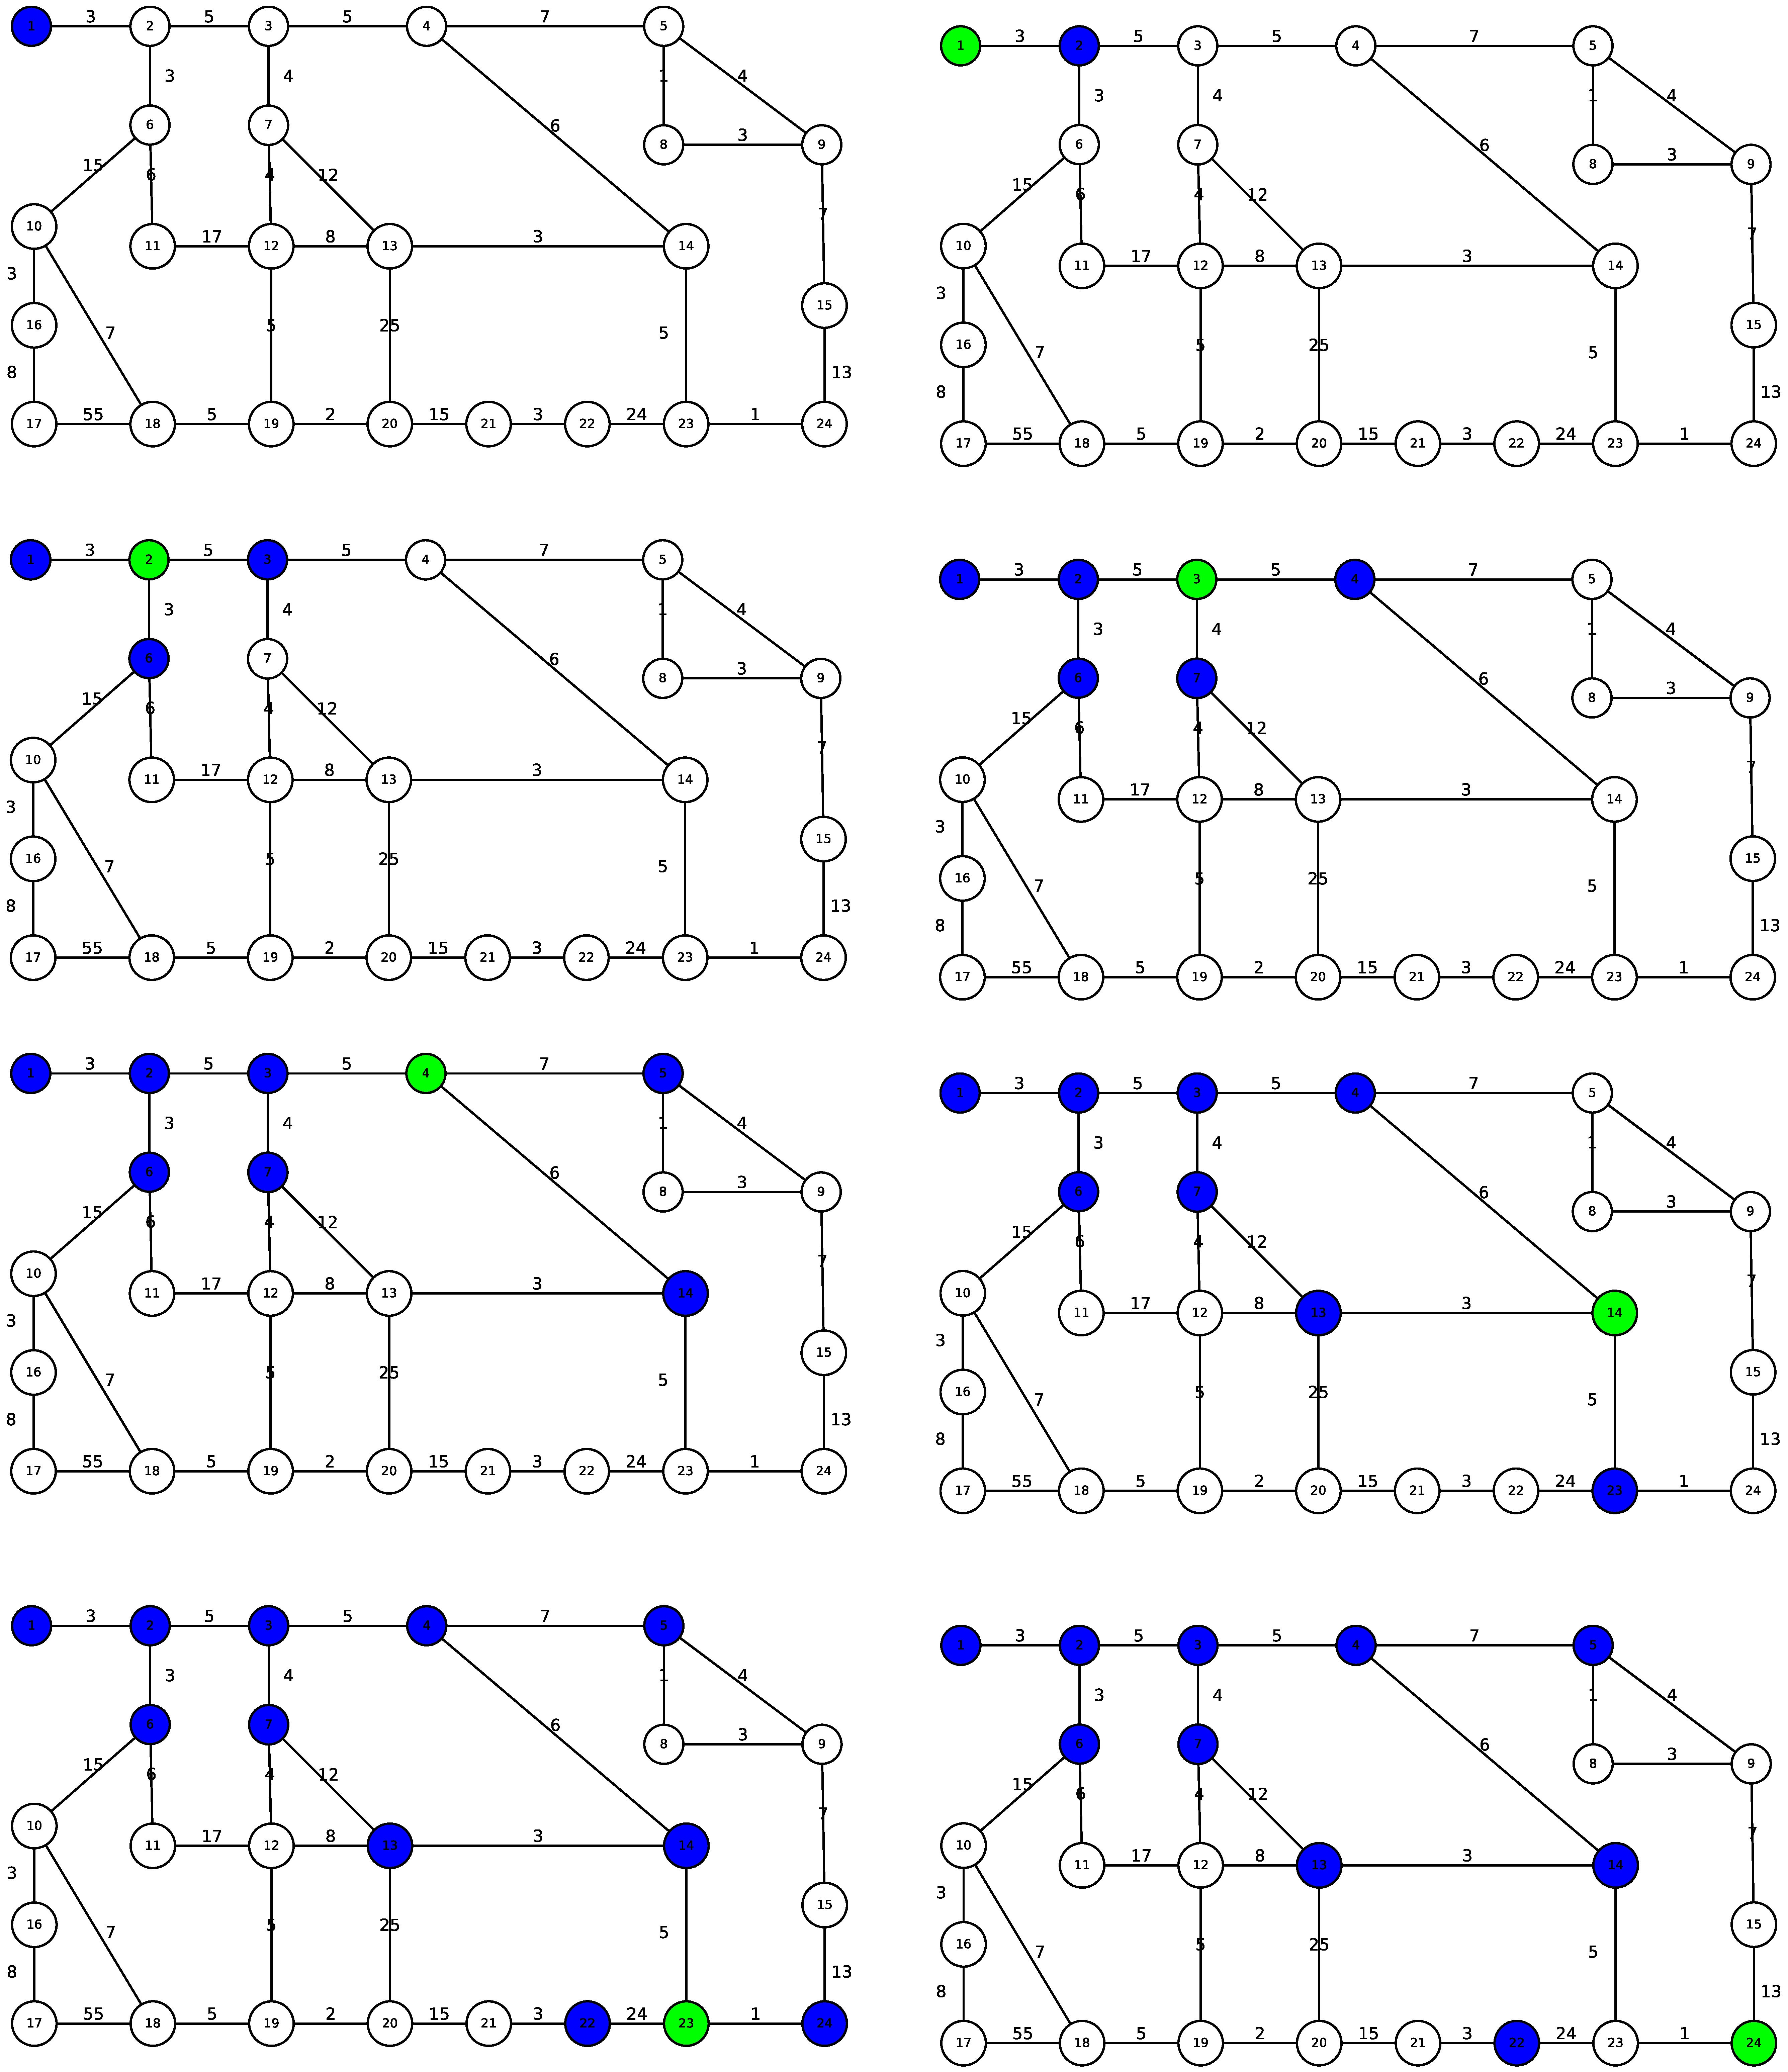
\includegraphics[ width={\textwidth} ]{pictures/tree_search}
\caption{A* star tree search algorithm}
\end{figure}

